\subsection{Login}
I dette afsnit vises design, bruger grænseflade, implementering og test for 'Login' viewet. For den fulde dokumentation henvises til Arkitektur og Design dokumentationens afsnit \ref{Design-sec:Login}.
\subsubsection{Design}
Sekvensdiagrammet for 'Login' viewet til Rambøll Tilsyn, kan ses på figur \ref{fig:LoginSekvens}. Figuren viser det logiske flow der sker når brugeren vil logge ind.
\begin{figure}[H] % (alternativt [H])
	\centering
	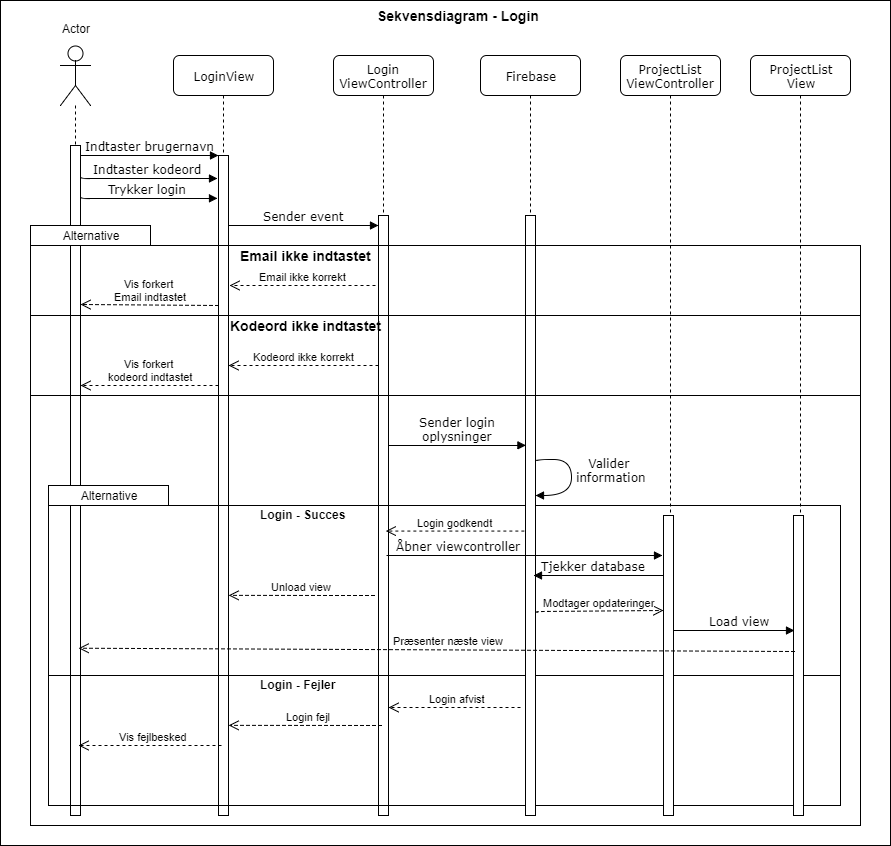
\includegraphics[height=15cm, width=15cm]{Design/Applikation/Login/LoginSekvensDiagram}
	\caption{Sekvensdiagram for Login i Rambøll Tilsyn.}
	\label{fig:LoginSekvens}
\end{figure}

\clearpage

\subsubsection{Grafisk brugergrænseflade}
I LoginViewet er der lavet felter til at bruger indtaster sit brugernavn og kodeord. Se figur \ref{fig:OpretBrugerView}
\begin{figure}[H] % (alternativt [H])
	\centering
	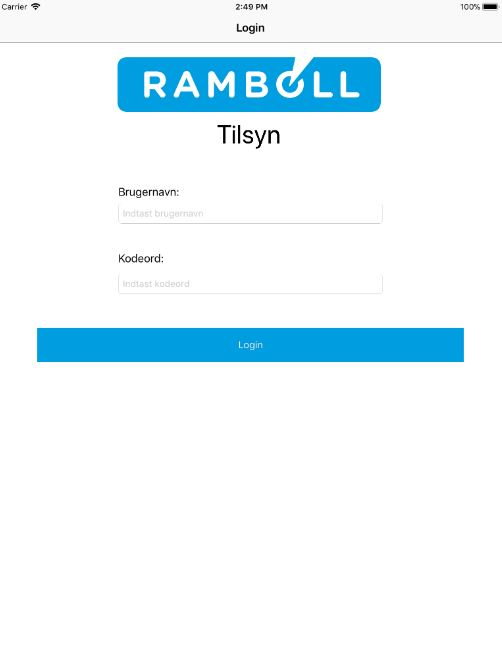
\includegraphics[height=12cm, width=10cm]{Design/Applikation/Login/LoginView}
	\caption{Login viewet som det er implementeret i Rambøll Tilsyn.}
	\label{fig:LoginView}
\end{figure}

\subsubsection{Implementering}

\subsubsection{Test}

\clearpage